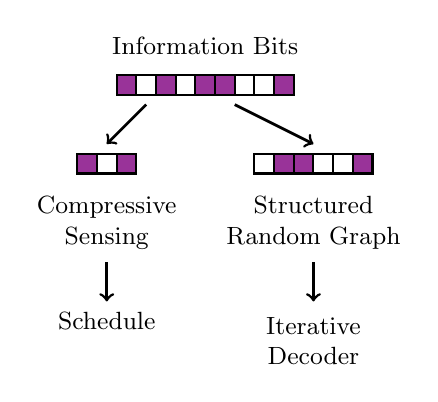
\begin{tikzpicture}
[font=\small, draw=black, line width=0.75pt,
bit0/.style={rectangle, draw, inner sep=0pt, minimum size=2.5mm},
bit1/.style={rectangle, draw, fill=violet!80, inner sep=0pt, minimum size=2.5mm},
entry0/.style={rectangle, draw, inner sep=0pt, minimum size=2.5mm},
entry1/.style={rectangle, draw, fill=lightgray, inner sep=0pt, minimum size=2.5mm},
entry2/.style={rectangle, draw, fill=darkgray, inner sep=0pt, minimum size=2.5mm},
symbol0/.style={rectangle, draw, fill=white, inner sep=0pt, minimum size=2.5mm},
symbol1/.style={rectangle, draw, fill=blue!50, inner sep=0pt, minimum size=2.5mm}]

\node[bit1] (s00) at (0.00,3.00) {};
\node[bit0] (s01) at (0.25,3.00) {};
\node[bit1] (s02) at (0.50,3.00) {};

\node[bit0] (s03) at (2.25,3.00) {};
\node[bit1] (s04) at (2.50,3.00) {};
\node[bit1] (s05) at (2.75,3.00) {};
\node[bit0] (s06) at (3.00,3.00) {};
\node[bit0] (s07) at (3.25,3.00) {};
\node[bit1] (s08) at (3.50,3.00) {};

\draw[->, line width=1pt]  (0.75,3.75) -- (0.25,3.25);
\draw[->, line width=1pt]  (1.875,3.75) -- (2.875,3.25);

\node[bit1] (info0) at (0.50,4) {};
\node[bit0] (info1) at (0.75,4) {};
\node[bit1] (info2) at (1.00,4) {};
\node[bit0] (info3) at (1.25,4) {};
\node[bit1] (info4) at (1.50,4) {};
\node[bit1] (info5) at (1.75,4) {};
\node[bit0] (info6) at (2.00,4) {};
\node[bit0] (info7) at (2.25,4) {};
\node[bit1] (info8) at (2.50,4) {};

\node (infobits) at (1.50,4.50) {Information Bits};
\node[align=center] (cs) at (0.25,2.25) {Compressive\\Sensing};
\draw[->, line width=1pt]  (0.25,1.75) -- (0.25,1.25);
\node[align=center] (schedule) at (0.25,1.00) {Schedule};

\node[align=center] (graph) at (2.875,2.25) {Structured\\Random Graph};
\draw[->, line width=1pt]  (2.875,1.75) -- (2.875,1.25);
\node[align=center] (peeling) at (2.875,0.75) {Iterative\\Decoder};
\end{tikzpicture}

